
\resizebox{\textwidth}{!}{

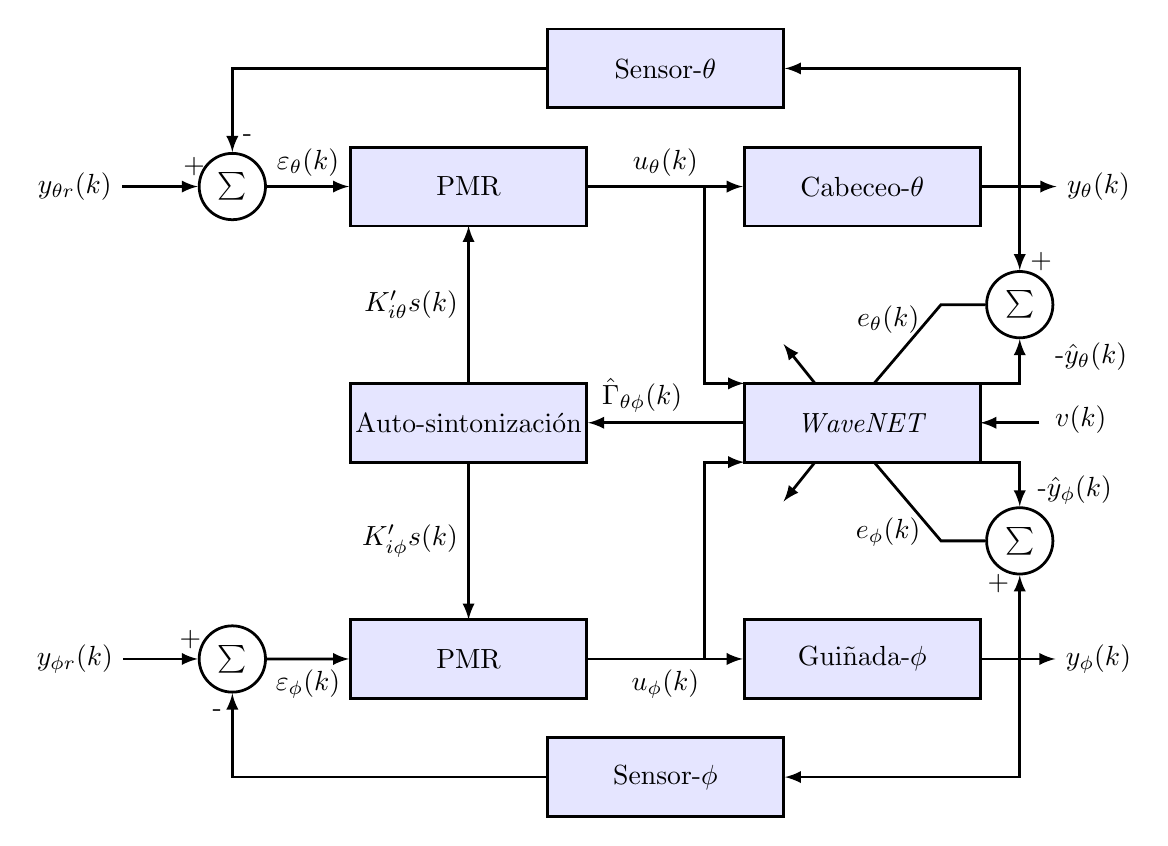
\begin{tikzpicture}[node distance = 5cm, auto, >=latex, line width = 1pt]
    \tikzstyle{block} = [draw, fill = blue!10, shape = rectangle, inner sep = 1pt, minimum height = 1cm, minimum width = 3cm]
    \tikzstyle{sum} = [draw, shape = circle, minimum size = 1em]

    \node[sum] (begin) at (0,0) {$\sum$};
    \node[] (start) [left of = begin, node distance = 2cm] {$y_{\theta r}(k)$};
    \node[block] (control) [right of = begin, node distance = 3cm] {PMR};
    \node[block] (process) [right of = control] {Cabeceo-$\theta$};
    \node[] (end) [right of = process, node distance = 3cm] {$y_{\theta}(k)$};
    \node[block] (gains) [below of = control, node distance = 3cm] {Auto-sintonización };
    \node[block] (rna) [below of = process, node distance = 3cm] {\textit{WaveNET}};
    \node[sum] (sum) at (10,-1.5) {$\sum$};
    \node[block] (sensor) at (5.5,1.5) {Sensor-$\theta$};
    
    \draw[->] (start) -- node[pos = 0.95] {+} (begin);
    \draw[->] (begin) -- node[pos = 0.50] {$\varepsilon_{\theta}(k)$} (control);
    \draw[->] (control) -- node {$u_{\theta}(k)$} (process);
        
    \draw[->] (3,-2.5) -- node {$K'_{i\theta}s(k)$} (3,-0.5);
    \draw[->] (10,0) -- node[pos = 0.9] {+} (sum);
    \draw[->] (9.25,-2.5) -| node[pos = 0.80, xshift = 1.5cm] {-$\hat{y}_{\theta}(k)$} (sum);
    \draw[->] (6.00,0) |- (6.5,-2.5);
    \draw[->] (10.25,-3) -- node[xshift = 0.90cm, yshift = 0.35cm]{$v(k)$} (9.5,-3);
    \draw[- ] (sum) -- (9,-1.5) -- node[pos = 0.5, above, xshift = -7pt]
        {$e_{\theta}(k)$} (8.15,-2.5);
    \draw[->] (7.4,-3.5) -- (7,-4);
    \draw[->] (10,0) |- (sensor);
    \draw[->] (sensor) -| node[pos = 0.9] {-} (begin);
    \draw[->] (process) -- (end);
    \draw[->] (rna) -- node[pos = 0.65, above] {$\hat{\Gamma}_{\theta\phi}(k)$} (gains);
    
    \node[sum] (begin2) at (0,-6) {\tiny $\sum$};
    \node[] (start2) [left of = begin2, node distance = 2cm] {$y_{\phi r}(k)$};
    \node[block] (control2) [below of = gains, node distance = 3cm] {PMR};
    \node[block] (process2) [below of = rna, node distance = 3cm] {\centering Guiñada-$\phi$};
    \node[] (end2) [right of = process2, node distance = 3cm] {$y_{\phi}(k)$};
    \node[block] (sensor2) at (5.5,-7.5) {Sensor-$\phi$};
    \node[sum] (sum2) at (10,-4.5) {$\sum$};
    
    \draw[<-] (3,-5.5) -- node {$K'_{i\phi}s(k)$} (3,-3.5);
    \draw[->] (start2) -- node[pos = 0.90] {+} (begin2);
    \draw[->] (begin2) -- node[pos = 0.50, below] {$\varepsilon_{\phi}(k)$} (control2);
    \draw[->] (control2) -- node[below] {$u_{\phi}(k)$} (process2);
    \draw[->] (6,-6) |- (6.5,-3.5);
    \draw[->] (10,-6) -- node[pos = 0.90] {+} (sum2);
    \draw[->] (9.25,-3.5) -| node[pos = 0.80, xshift = 0.7cm, below, yshift = 0.3cm] {-$\hat{y}_{\phi}(k)$} (sum2);
    \draw[->] (10,-6) |- (sensor2);
    \draw[->] (sensor2) -| node[pos = 0.90] {-} (begin2);
    \draw[->] (process2) -- (end2);
    
    \draw[- ] (sum2) -- (9,-4.5) -- node[pos = 0.5, above, xshift = -7pt, yshift = -0.7cm] {$e_{\phi}(k)$} (8.15,-3.5);
    \draw[->] (7.4,-2.5) -- (7,-2);
\end{tikzpicture}}